
\begin{frame}[allowframebreaks]{Objectives}
		
    \begin{enumerate}[\textbullet]
        \item Write a class for the EnKF in C++, inspired by the EnKF written in Python (FilterPy); Test the algorithm.
        \item To read the following article :
        \begin{itemize}
            \item Fundamentals Of Building Performance Simulation By Beausoleil-Morrison
        \end{itemize}
        
    \item Understand the heat equation and what are the phenomena involved in the modification of the temperature of a building (conduction, convection, radiation).
    \item Realize with Gmsh the geometry of the figure.
    \item Write the mathematical problem to be solved if we want to simulate an office then realize the simulation using Feel++ toolboxes.
    \item Introduce data assimilation using the sensor and correct the simulation.
    \end{enumerate}
\end{frame}




\begin{frame}{Introduction to data assimilation}
Data assimilation is widely used in:
\begin{enumerate}[\textbullet]
       \item weather forecasting
       \item ocean simulation
\end{enumerate}	 
      The main idea of computational data assimilation is to combine:
\begin{enumerate}[\textbullet]
       \item a model
       \item some observations
\end{enumerate}	 
The best estimation:
$$x^a=Lx^b+Ky^0$$
with $x^a$ the analyzed state, $x^b$ the state of the model and $y^0$ the observations.
\end{frame}
\subsection{Theory}

\begin{frame}[allowframebreaks]{Statistical approach : Derivation of the Kalman filter}
   The Kalman filter method consists in looking for $x^a$ as linear combination of our model and our observations.
   \begin{equation*}
       x^a=x^b+K(y-x^b)
       \label{eq1}
   \end{equation*}
   with K the gain matrix.
\newpage
    The Kalman filter method consists in looking for $x^a$ as linear combination of our model and our observations.
   \begin{equation}
       x^a=x^b+K(y-x^b)
       \label{eq1}
   \end{equation}
   with K the gain matrix.
   \newline Let’s consider that true state $x^t$ exists:
   \begin{equation}
       x^a-x^t=x^b-x^t+K(y-x^t-x^b+x^t)
   \end{equation}
   Errors: \qquad $\epsilon^a=x^a-x^t,\qquad \epsilon^b=x^b-x^t, \qquad \epsilon^y=y-x^t$ \\
   One realisation of these errors :$ \quad \epsilon^a=\epsilon^b+K(\epsilon^y-\epsilon^b)$
   Many realisation of these errors + sample average :
   \begin{equation}
       <\epsilon^a>=<\epsilon^b>+K(<\epsilon^y>-<\epsilon^b>)
   \end{equation}
\end{frame}
\begin{frame}{Kalman filter in one-dimension}

   Analysis error variance as low as possible.
   \newline Minimize $<(\epsilon^a)^2>$ with respect to $K$ :
   $$<(\epsilon^a)^2>=<(\epsilon^b)^2>+K^2<(\epsilon^y-\epsilon^b)^2>+2K<\epsilon^b(\epsilon^y-\epsilon^b)^2>$$
   The errors in the background and observation are uncorrelated.
   $$K=\frac{<(\epsilon^b)^2>}{<(\epsilon^b)^2>+<(\epsilon^y)^2>} \Rightarrow K=\frac{(\sigma^b)^2}{(\sigma^b)^2+(\sigma^y)^2} $$
   $(\sigma^y)^2$ the observation error variance, \newline $(\sigma^b)^2$ the background or model error variance.

\end{frame}
   
\begin{frame}{Kalman filter in multi-dimensional case}
   Now that we have explained the method for finding $x^a$ let's try to generalize our formula in a \textbf{multi-dimensional case}.

   $$\left\{\begin{aligned}
     &x^a=(I-KH)x^b+Ky^0=x^b+K(y^0-H(x^b)) \\
           &K=BH^T(HBH^T+R)^{-1} \\
    \end{aligned}\right.$$
   With $K$ the gain or weight matrix.
   The Best Linear Unbiased Estimator (BLUE).
   \begin{figure}[H]
       \pgfimage[width=0.4\linewidth]{images/enkf/schema_kalman_filter.png}
       \caption{Kalman Filter}
   \end{figure}
\end{frame}
\begin{frame}{Ensemble Kalman Filter}
   The ENKF method consists in using the Kalman filter in non-linear system.
   \newline We apply the Kalman filter on several state samples $x_1,x_2,..,x_{m}$.
   $$x_i^a=x_i^f+K[y-h(x_i^f)]$$
   with $h(x_i^f)$ the observation operator.
   We can also define the Kalman gains: 
   $$K=P^f H^T(HP^f H^T+R)^{-1}$$
   For exemple we can estimate the
   forecast error covariance matrix as:
   $$P^f=\frac{1}{m-1}\sum_{i=1}^{m}(x_i^f-\bar{x}^f)(x_i^f-\bar{x}^f)^T~~\text{with}~~\bar{x}^f=\frac{1}{m}\sum_{i=1}^{m}x_i^f $$ .
\end{frame}
\begin{frame}{Comparing Cpp results with Python}
	\centering
$\sigma=12, \quad b=6, \quad r=12, \quad X_0=(-10,-10,25), \quad t_0=0, \quad T=1$
\begin{minipage}{0.48\linewidth}
	\begin{figure}[H]
		\pgfimage[width=0.9\linewidth]{images/enkf/Comparaison_python.jpg}
		\caption{Result with Filterpy}
	\end{figure}
\end{minipage}
\begin{minipage}{0.48\linewidth}
	\begin{figure}[H]
		\pgfimage[width=0.9\linewidth]{images/enkf/Comparaison_cpp.jpg}
		\caption{Result with Cpp}
	\end{figure}
\end{minipage}
\end{frame}
\subsection{Integrate data assimilation to Feel++}
\begin{frame}[allowframebreaks]{The context}
\begin{itemize}
    \item Our goal is to make the simulation of an office in the university of Strasbourg in which we have 10 sensors to measure the temperature.\\
    \item We want to apply data assimilation and use our sensors to correct the temperature of the room.
\end{itemize}

\begin{minipage}{0.48\linewidth}
    \begin{figure}
        \centering
        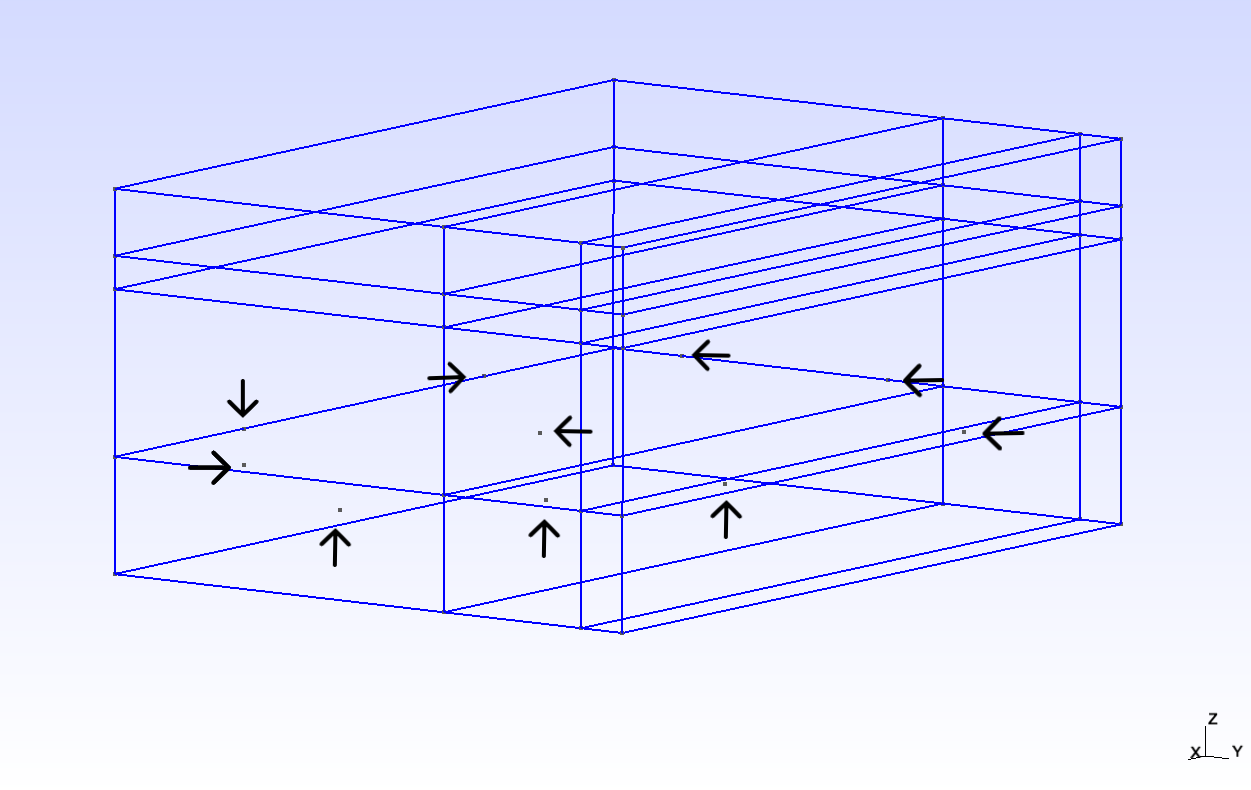
\includegraphics[width=\linewidth]{"images/enkf/Maillage_1.jpg"}
        \caption{Mesh of the office that we will use for the simulation.}
    \end{figure}
\end{minipage} \;
\begin{minipage}{0.48\linewidth}
    \begin{figure}
        \centering
        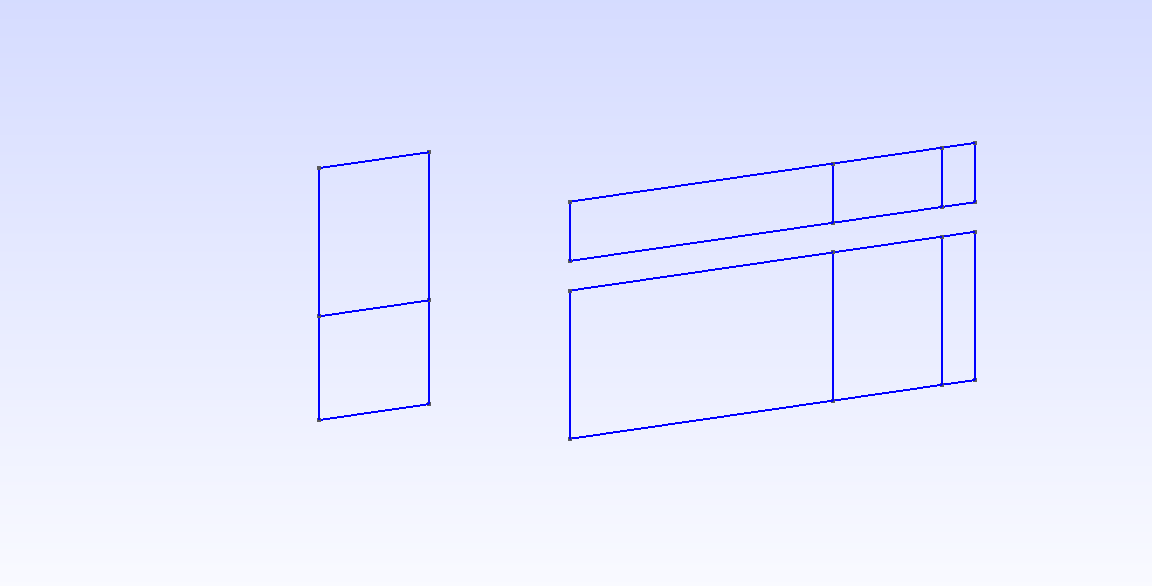
\includegraphics[width=\linewidth]{"images/enkf/Maillage_2.jpg"}
        \caption{Visualization of windows and door in the mesh.}
    \end{figure}
\end{minipage}
\newpage
\begin{itemize}
    \item Heat equation with convective effects\\
    $$\rho C_p((\frac{\partial T}{\partial t})+u . \nabla T)-\nabla .(k \nabla T)=Q$$
    Which is completed with boundary conditions and initial value.
    \newline
    \newline
\renewcommand{\arraystretch}{2}
\begin{tabular}{|R{2cm}|C{2.5cm}|L{2.5cm}|L{2.5cm}|}
\hline
$\rho$ & Air density & $Kg.m^
{-3}$ & 1.125  \\[0.5cm]
\hline
$C_p$ & Specific heat & $J/KgK$ & 1004 \\[0.5cm]
\hline
$k$ & Conductivity & $W/mK$ & 0.025  \\[0.5cm]
\hline
$u$ & Fluid velocity & $m.s^{-1}$ & unknown \\[0.5cm]
\hline
\end{tabular}
\newpage
\item Equation of the air motion (Navier-Stokes).
 $$\left\{\begin{aligned} 
        &\rho (\frac{\partial u}{\partial t}+u.\nabla u)-\nabla.(\mu \nabla u)+\nabla P =-\rho_0 \beta(T-T_{ref})g\\
        &\nabla . u=0 \\
    \end{aligned}\right.$$
\renewcommand{\arraystretch}{2}
\begin{tabular}{|R{1cm}|C{5cm}|L{1.5cm}|L{1.5cm}|}
\hline
$\rho$ & fluid density & $Kg.m^
{-3}$ & 1.125 \\[0.7cm]
\hline
$u$ & fluid velocity & $m.s^{-1}$ & unknown \\[0.7cm]
\hline
$\beta$ & coefficient of thermal expansion & $K^
{-1}$ &  0.0034 \\[0.7cm]
\hline
$\mu$ & dynamic viscosity & $Pa.s$ & $1.81e^{-5}$\\[0.7cm]
\hline
$g$ & gravitational acceleration & $m.s^{-2}$ & $9.8$\\[0.7cm]
\hline
\end{tabular}
\end{itemize}
\newpage
\begin{minipage}{0.30\linewidth}
    \begin{figure}
        \centering
        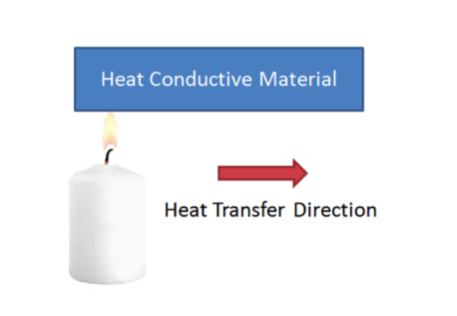
\includegraphics[width=1.2\linewidth]{images/enkf/conduction.png}
        \caption{Conduction}
    \end{figure}
\end{minipage} \;
\begin{minipage}{0.30\linewidth}
    \begin{figure}
        \centering
        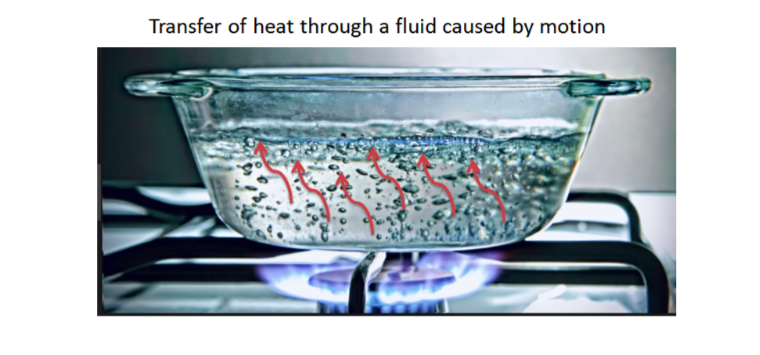
\includegraphics[width=1.2\linewidth]{images/enkf/convection.png}
        \caption{Convection}
    \end{figure}
\end{minipage}
\begin{minipage}{0.35\linewidth}
    \begin{figure}
        \centering
        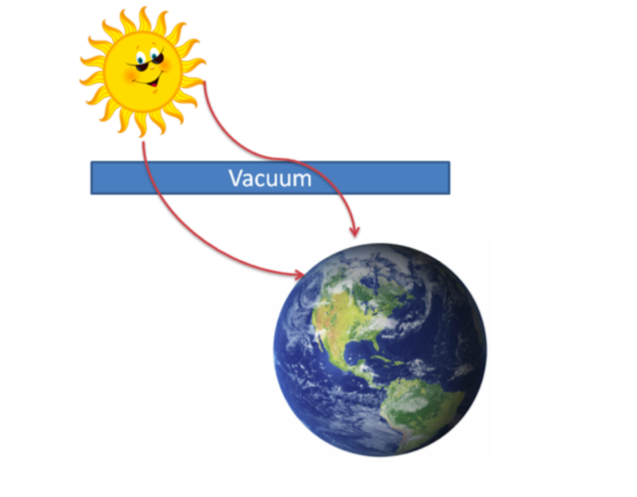
\includegraphics[width=1.2\linewidth]{images/enkf/radiation.png}
        \caption{Radiation}
    \end{figure}
\end{minipage}

\end{frame}
\begin{frame}[allowframebreaks]{Simulation}
\begin{minipage}{0.48\linewidth}
    \begin{figure}
        \centering
        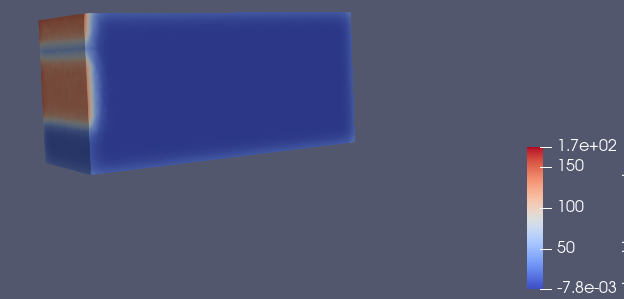
\includegraphics[width=\linewidth]{"images/enkf/Simulation_1.jpg"}
        \caption{Visualization of the simulation made with the toolbox heat (4th second) .}
    \end{figure}
\end{minipage} \;
\begin{minipage}{0.46\linewidth}
    \begin{figure}
        \centering
        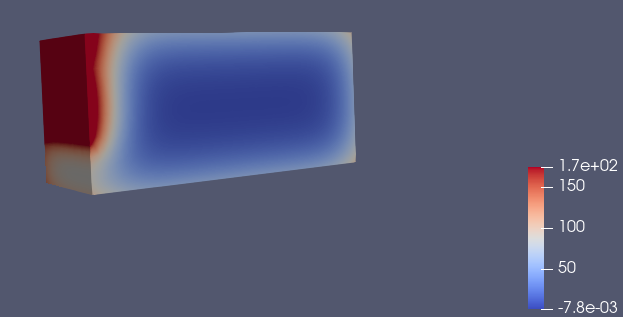
\includegraphics[width=\linewidth]{"images/enkf/Simulation_2.jpg"}
        \caption{Visualization of the simulation made with the toolbox heat (38th second) .}
    \end{figure}
\end{minipage}
\begin{itemize}
    \item For this simulation we do not consider the convection, but we increase k (Conductivity) in order to visualize the temperature increase in the room.
\end{itemize}

\end{frame}
    
\begin{frame}{Continuation of the project}
	\textbf{Goal :} Try to apply data assimilation to our model using our sensors as observation to correct the simulation.
\end{frame}



